\subsection{Underchapter Example}
\label{subsec:underchapterexample}

Die Gestalt von Propellern kann durch viele 2D-Profile beschrieben werden. 2D-Profile gleichen dem Querschnitt eines Flügels. Durch den geringeren Druck auf der Oberseite des Profils resultieren Kräfte, die das Profil hoch drücken (siehe Kapitel \ref{subsec:momentumtheorie}, Einschub Bernoulli) oder im Falle des Propellers, Schub erzeugen. Für jedes Profil können die Kräfte dargestellt werden.

\vspace{0.05cm}

\begin{figure}[htb!]
\begin{center}
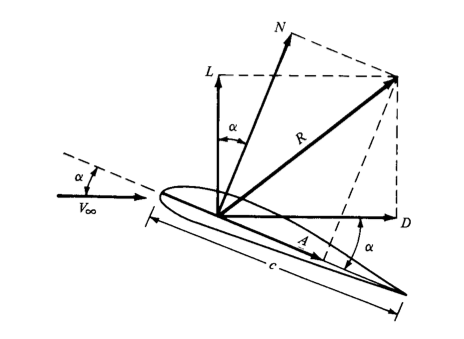
\includegraphics[width=0.48\textwidth]{airfoilKraefte}
\caption[Wirksame aerodynamische Kräfte an einem Profil]{Wirksame aerodynamische Kräfte an einem Profil \cite{aeroKraefte}. Die Auftriebskraft $L$ wirkt beim Propeller als Schub und die Widerstandskraft $D$ als Drehmoment.}
\label{fig:airfoilKraefte}
\end{center}
\end{figure}

\vspace{0.05cm}

In Abbildung \ref{fig:airfoilKraefte} sind die verschiedenen Kräfte dargestellt. $V_\infty$ stellt die Geschwindigkeit der Luft weit weg vom Körper dar. Die Kraft $R$ setzt sich zusammen aus der Auftriebskraft $L$ ('lift') und der Widerstandskraft $D$ ('drag'), wobei $L$ senkrecht zu $V_\infty$ steht und $D$ in die gleiche Richtung zeigt wie $V_\infty$.
Die Sehnenlänge $c$ ('chord') definiert die Länge des Profils von der Profilspitze bis zur Hinterkante. Dabei steht die Kraft $N$ senkrecht zu $c$ und $A$ in Richtung $c$. Der Winkel $\alpha$ ist der Winkel zwischen $V_\infty$ und $c$.
Über trigonometrische Funktionen können die Kräfte $N$ und $A$ folgendermassen beschrieben werden:
\newpage

